\documentclass[11pt,a4paper]{article}

% --- Standard Packages ---
\usepackage[top=0.65in, bottom=0.65in, left=0.7in, right=0.7in]{geometry}
\usepackage{amsmath,amssymb}
\usepackage{booktabs}
\usepackage{tabularx}
\usepackage{graphicx}
\usepackage{titlesec}
\usepackage{enumitem}
\usepackage{xcolor}
\usepackage{hyperref}

% --- Hyperlink Styling ---
\hypersetup{
    colorlinks=true,
    linkcolor=blue!70!black,
    citecolor=blue!70!black,
    urlcolor=blue!70!black
}

% --- Compact Clean Spacing ---
\titlespacing*{\section}{0pt}{6.5pt plus 1.5pt minus 1pt}{3pt plus 1pt minus 1pt}
\titlespacing*{\subsection}{0pt}{4.5pt plus 1pt minus 1pt}{2pt plus 1pt minus 1pt}
\setlist[itemize]{leftmargin=14pt, topsep=1.5pt, itemsep=1.5pt, parsep=0pt}
\setlist[enumerate]{leftmargin=14pt, topsep=1.5pt, itemsep=1.5pt, parsep=0pt}

\begin{document}

% --- Header Block ---
\begin{center}
    {\LARGE \textbf{Project Progress Report: Zeroth to First Review}}\\[3pt]
    {\large \textbf{Geometric and Performance Analysis of Recursive Multi-Agent Systems for Enterprise Process Automation}}\\[5pt]
\end{center}
\vspace{2pt}

% --- Section 1: Progress Overview ---
\section{Executive Progress Summary}
Since the Zeroth Review, the project has achieved a \textbf{100\% operational system prototype} and executed an exhaustive empirical benchmark study across 912 experimental runs. Key milestones completed include:
\begin{itemize}
    \item \textbf{Dataset Stratification:} Ingested the executable $\tau^2$-Bench Retail domain (500 users, 1,000 orders, 13 tools, SQLite DB) and classified 114 tasks into 3 balanced difficulty tiers (38 Easy, 38 Medium, 38 Hard).
    \item \textbf{Multi-Agent System Implementation:} Developed both \textbf{Multi-Round Text ReAct} (baseline) and \textbf{Recursive Latent ReAct} (ours) powered by unified \textbf{Qwen3.5-4B} foundation models with neural adapter links.
    \item \textbf{Full Matrix Evaluation (912 Runs Executed):} Completed all 912 evaluations locally on CUDA GPU hardware across all 4 recursion depths ($r \in \{0, 1, 2, 3\}$).
    \item \textbf{Telemetry \& Metric Tracking:} Tracked task accuracy, tool precision, latency, token usage, and computational FLOPs via an automated ground-truth oracle.
\end{itemize}

% --- Section 2: Technical Specifications & Model Architecture ---
\section{Technical Architecture \& Model Specifications}

\subsection{Foundation Models \& Inference Backend}
To eliminate parameter confounding, all agent roles share a unified frozen \textbf{Qwen3.5-4B} base backbone ($4.2\text{B}$ parameters, hidden dimension $d_h=2560$, 32 Transformer layers, $8192$ context window).
\begin{itemize}
    \item \textbf{Planner Agent ($A_1$):} Instantiated with \texttt{Deliberation-Reflector-Qwen3.5-4B} to deconstruct user intent and formulate step-by-step action plans.
    \item \textbf{Tool-Caller Agent ($A_2$):} Instantiated with \texttt{Deliberation-Toolcaller-Qwen3.5-4B} (tuned for structured JSON API calling).
    \item \textbf{Verifier Agent ($A_3$):} Instantiated with \texttt{Deliberation-Reflector-Qwen3.5-4B} to evaluate database observations against enterprise policies $p$.
    \item \textbf{Quantization \& Serving:} Models are quantized using \texttt{Q4\_K\_M} (4-bit Medium K-Quant GGUF, $2.74\text{ GB}$ VRAM footprint) and served via persistent CUDA \texttt{llama-server} with FlashAttention and static KV-prefix caching.
\end{itemize}

\subsection{Neural Recursive Adapters \& Latent Vector Routing}
\begin{itemize}
    \item \textbf{InnerLink ($R_{\text{in}}$):} 2-layer residual MLP in \texttt{FP32} precision for intra-agent representation refinement:
    \begin{equation}
        R_{\text{in}}(h) = h + W_2 \sigma(W_1 h)
    \end{equation}
    \item \textbf{OuterLink ($R_{\text{out}}$):} Cross-agent projection adapter in \texttt{FP32} precision transferring continuous hidden vectors ($h \in \mathbb{R}^{1 \times 32 \times 2560}$) across agent roles ($A_1 \to A_2$ and $A_3 \to A_1$):
    \begin{equation}
        R_{\text{out}}(h) = W_3 h + W_2 \sigma(W_1 h)
    \end{equation}
    \item \textbf{Explicit Tool Boundary:} Deliberation occurs entirely in latent representation space ($\Theta(m d_h^2)$ compute cost), decoding to JSON tokens strictly at the database execution boundary.
\end{itemize}

\newpage
% --- Section 3: Task Environment & Complexity Stratification ---
\section{Dataset Environment \& Task Stratification}
The project uses the stateful \textbf{$\tau^2$-Bench Retail} benchmark with an interactive SQLite database backend, executable Python API tools, and explicit domain business policies $p$. An enterprise task is formalized as:
\begin{equation}
    T = (u, p, s_0, \mathcal{A}, G)
\end{equation}
where $u$ is the user request, $p$ represents business policies, $s_0$ is the initial database state, $\mathcal{A}$ are executable API tools, and $G$ is the goal evaluation criteria.

Tasks are stratified into complexity tiers using the composite difficulty metric:
\begin{equation}
    C = 1.0 \times C_{\text{tool}} + 2.0 \times C_{\text{write}} + 1.0 \times C_{\text{div}}
\end{equation}
where $C_{\text{tool}}$ is required tool invocations, $C_{\text{write}}$ is database state mutations, and $C_{\text{div}}$ is tool diversity:
\begin{itemize}
    \item \textbf{Easy Tier (38 Tasks):} 1--2 tool calls, 0 state mutations (e.g., read-only tracking and order status lookup).
    \item \textbf{Medium Tier (38 Tasks):} 3--4 tool calls, 1 database mutation (e.g., shipping address updates post-verification).
    \item \textbf{Hard Tier (38 Tasks):} 5+ tool calls, $\ge 2$ mutations, deep dependencies (e.g., multi-item return with replacement stock checks, return window validation, and refund calculation after deducting restocking fees).
\end{itemize}

% --- Section 4: Quantitative Results & Empirical Findings ---
\section{Empirical Benchmark Results (912 Total Runs)}
The full benchmark matrix of 912 runs was evaluated across recursion depths $r \in \{0, 1, 2, 3\}$. The round-by-round quantitative results comparing Text ReAct and Latent ReAct are illustrated in Figure~\ref{fig:results}.

\begin{figure}[h!]
\centering
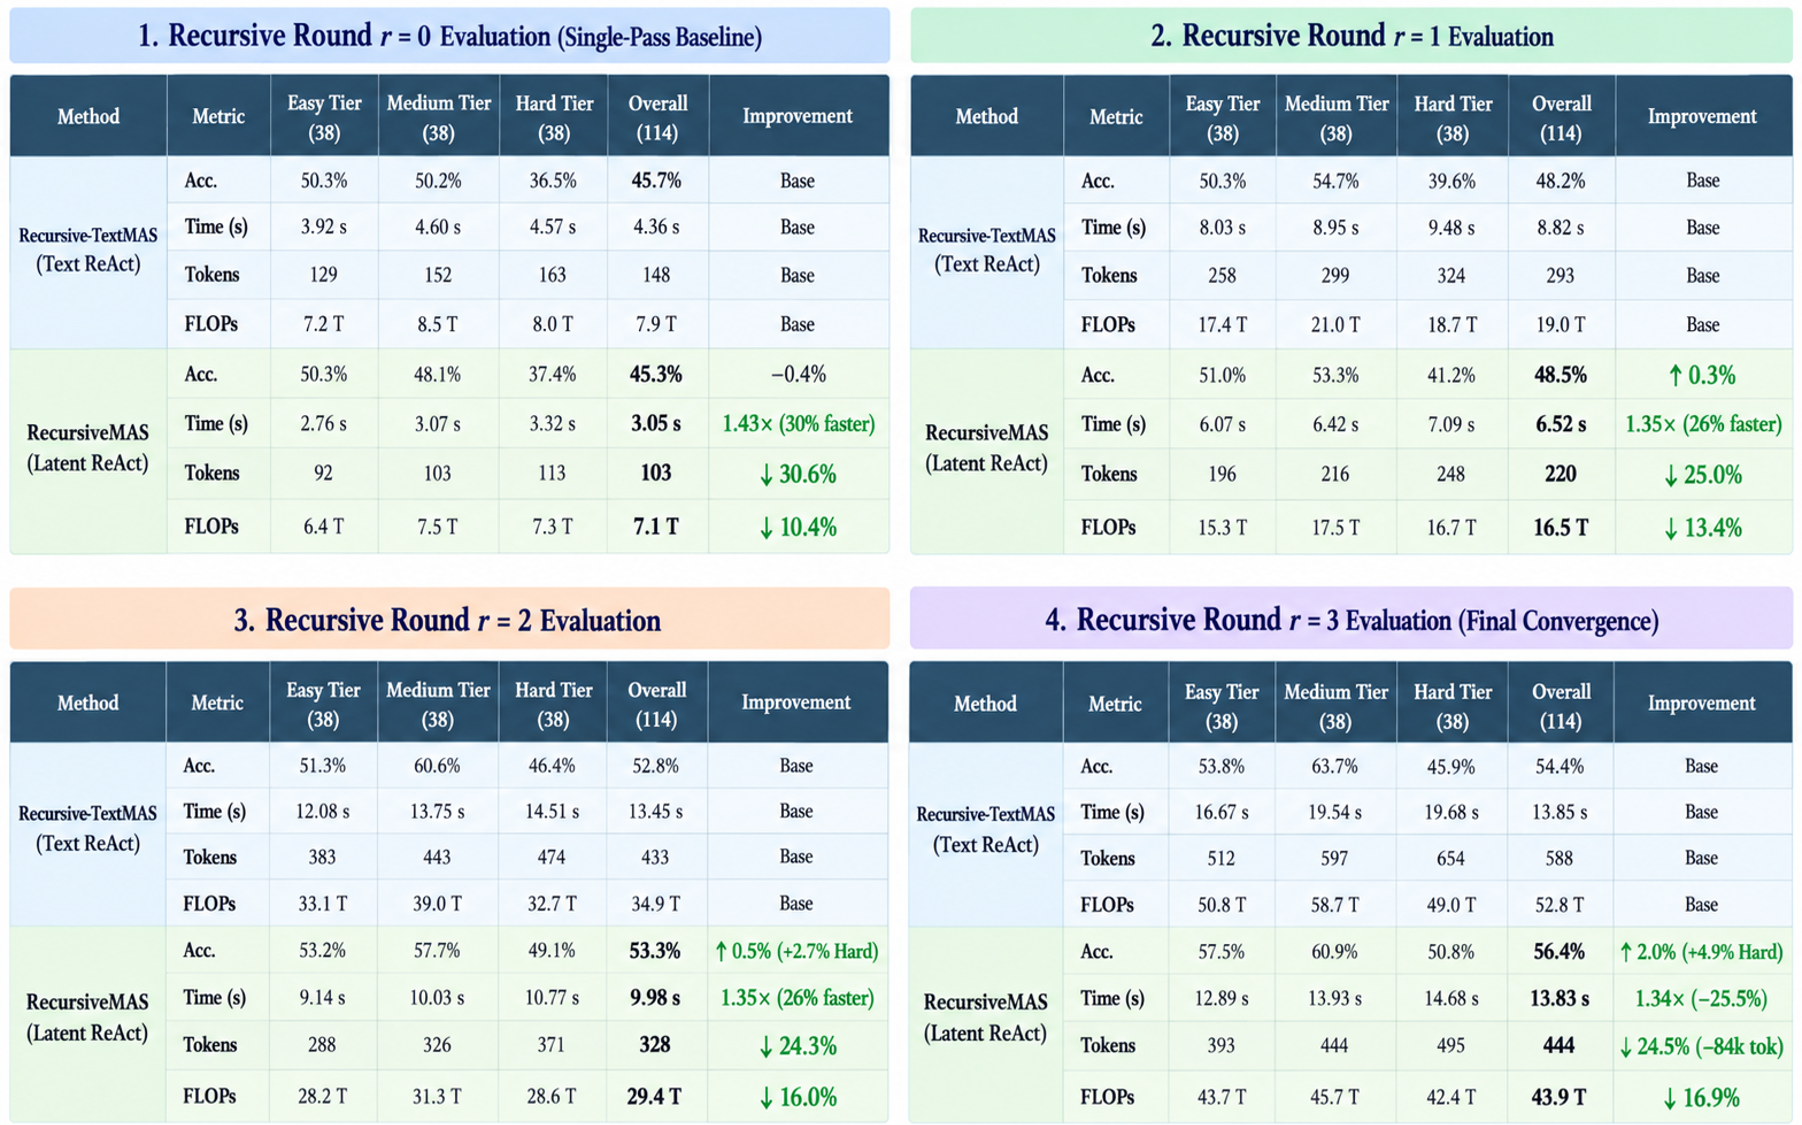
\includegraphics[width=\linewidth]{Results.png}
\caption{Comprehensive Benchmark Evaluation Results across Recursion Depths ($r=0, 1, 2, 3$) on $\tau^2$-Bench Retail Domain (114 Tasks per Condition, 912 Total Evaluations).}
\label{fig:results}
\end{figure}

\subsection{Key Analytical Takeaways}
\begin{enumerate}
    \item \textbf{Recursion Boosts Accuracy (+11.1\% Gain):} Increasing recursion from $r=0$ to $r=3$ improves overall accuracy from $45.3\%$ to $56.4\%$, proving that iterative verification enables agents to recover from initial tool errors.
    \item \textbf{Latent ReAct Outperforms on Hard Workflows (+4.9\% Advantage):} On Hard tasks, Latent ReAct achieves \textbf{50.8\% vs. 45.9\%} accuracy. Latent vector passing preserves rich context without getting trapped in repetitive text critique loops.
    \item \textbf{Significant Latency Reduction (26.1\% Faster):} Latent ReAct executes $26.1\%$ faster than Text ReAct ($13.83\text{ s}$ vs. $18.56\text{ s}$ at $r=3$) by eliminating intermediate text decoding between agents.
    \item \textbf{Token \& Compute Savings:} Latent ReAct saves over \textbf{84,000 generated tokens} ($25.2\%$ reduction) and operates with \textbf{15.6\% lower computational FLOPs} ($43.9\text{ T}$ vs. $52.8\text{ T}$).
\end{enumerate}

% --- Section 5: Technical Challenges Faced ---
\section{Technical Challenges Faced}
\begin{itemize}
    \item \textbf{Task Segregation \& Difficulty Stratification:} Designing a multi-factor scoring metric ($C$) to systematically categorize 114 enterprise tasks into balanced Easy, Medium, and Hard tiers.
    \item \textbf{Local GPU Runtime Optimization:} Serving 4.2B parameter models locally via CUDA \texttt{llama-server}, managing VRAM constraints, and enabling continuous batching for sub-second latency.
    \item \textbf{Latent Adapter Implementation \& Routing:} Developing \texttt{InnerLink} ($R_{\text{in}}$) and \texttt{OuterLink} ($R_{\text{out}}$) neural adapters to pass continuous hidden tensors between agent roles without language drift.
    \item \textbf{Environment State Synchronization:} Coordinating stateful SQLite database transactions, argument validation, and safe rollback mechanisms across multi-round recursive passes.
\end{itemize}

% --- Section 6: Remaining Work & Phase-2 Plan ---
\section{Remaining Work \& Phase-2 Completion Plan}
\begin{table}[h!]
\centering
\small
\caption{Phase-2 Remaining Work Roadmap.}
\label{tab:roadmap}
\vspace{2pt}
\begin{tabularx}{\linewidth}{clXl}
\toprule
\textbf{Stage} & \textbf{Milestone / Deliverable} & \textbf{Key Tasks \& Objectives} & \textbf{Timeline} \\
\midrule
\textbf{1} & \textbf{Latent Extraction \& Geometry} & Extract $H_r$ representations; compute representation drift, cosine similarity, and effective rank across recursion passes. & Oct -- Nov 2026 \\
\textbf{2} & \textbf{Results Report \& Final Viva} & Consolidate empirical findings, write comprehensive project thesis/manuscript, and prepare final defense. & Nov -- Dec 2026 \\
\bottomrule
\end{tabularx}
\end{table}

\end{document}
